From the given information, 
% Given pdf of X as
% \begin{align}
%     f_{X}(x)=\begin{cases} 
%             \frac{2x}{\pi^2}  &  0<x<\pi\\
%             0 & \text{otherwise}
%             \end{cases} 
% \end{align}
\begin{align}
    F_X(x) &= \pr{X\leq x}\\
    &=\begin{cases} 
            0 & x\le 0\\
            \frac{x^2}{\pi^2}  &  0<x<\pi\\
            1 & x\ge \pi
            \end{cases}
            \label{trans/1/a}
\end{align}
after integration.  Consequently, 
\begin{align}
    F_Y(y) &= \pr{Y\leq y}\\
     &= \pr{\sin{X}\leq y}
\end{align}
From Fig. \ref{trans/1/plot}, 
\begin{figure}[!ht]
    \centering
    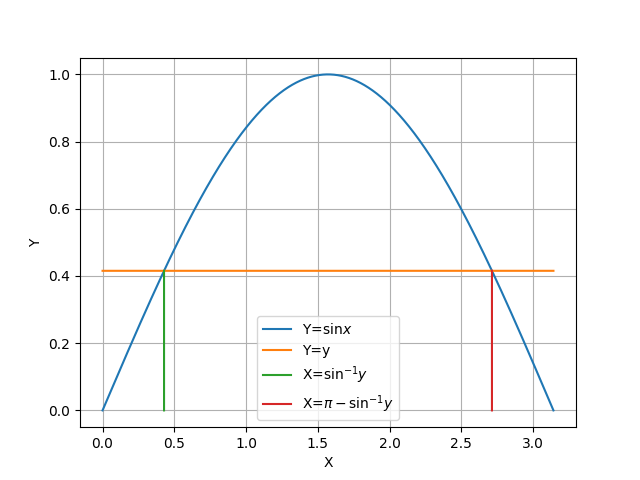
\includegraphics[width=\linewidth]{trans/solutions/1/plot.png}
    \caption{$Y=\sin X$ plot}
    \label{trans/1/plot}
\end{figure}
%
\begin{multline}
    \sin{X}\leq y 
    \\
    \implies \cbrak{X\leq \sin^{-1}{y} \cup X\geq \pi-\sin^{-1}{y}} 
\end{multline}
\begin{align}
    \implies F_Y(y) &= \pr{X\leq \sin^{-1}{y}} \nonumber \\
    & \quad +\pr{X\geq \pi-\sin^{-1}{y}}\\
     &= F_X(\sin^{-1}{y}) \nonumber \\
     & \quad +1-\pr{X\leq \pi-\sin^{-1}{y}}\\
    \implies F_Y(y) &= 1 + F_X(\sin^{-1}{y})-F_X(\pi-\sin^{-1}{y})
    \label{trans/1/b}
\end{align}
Substituting from  \eqref{trans/1/a} in \eqref{trans/1/b}
\begin{align}
 F_Y(y) &= \frac{\brak{\sin^{-1}{y}}^2}{\pi^2}+1-\frac{\brak{\pi-\sin^{-1}{y}}^2}{\pi^2}\\
    &= \frac{2\sin^{-1}{y}}{\pi}
\end{align}
%
\begin{align}
    \therefore     f_Y(y) &= \diff{F_Y(y)}{y}\\
    &= \frac{2}{\pi\sqrt{1-y^2}}
\end{align}
Hence, option(D) is correct.
